\documentclass[reprint,amsmath,amssymb,aps,twoside]{revtex4-2}


\usepackage{graphicx}
\usepackage{amsmath,amssymb,amsfonts}
\usepackage{dcolumn}
\usepackage{bm}
\usepackage{siunitx}
\sisetup{separate-uncertainty=true}
\usepackage[colorlinks,allcolors=blue]{hyperref}
\usepackage{cleveref}
\crefname{equation}{}{}
\crefname{figure}{Fig.}{Figs.}
\crefname{table}{Table}{Tables}
\usepackage{svg}
\usepackage{tikz,pgfplots}
% set PDF metadata
\hypersetup{%
pdftitle={Investigating Newton's first law in a pulley system},
pdfauthor={Andrew Barone, Alexander Gut, Rishith Kilaru, and Shrikar Swami},
}
\usepackage{fancyhdr}
\pagestyle{fancy}
\fancyhf{}
\fancyhead[RE,RO]{J S\&E \textbf{1}, 9--10 (2024)}
\fancyhead[LO]{Barone et al.}
\fancyhead[LE]{Investigating Newton's first law}
\fancyfoot[C]{\thepage}
\fancypagestyle{mytitlepage}{
\fancyhf{}
\fancyhead[C]{Journal of Science \& Engineering \textbf{1}, 9--10 (2024)}
\fancyfoot[C]{\thepage}
}



\begin{document}
\setcounter{page}{9}
\title{Investigating Newton's first law in a pulley system}
\author{Andrew Barone}
\email{Contact author: 425abarone@frhsd.com}
\author{Alexander Gut}
\author{Rishith Kilaru}
\email{Contact author: 426rkilaru@frhsd.com}
\altaffiliation{Science \& Engineering Magnet Program, \href{https://manalapan.frhsd.com/}{Manalapan High School}, Englishtown, NJ 07726 USA}
\author{Shrikar Swami}
\affiliation{\href{https://manalapan.frhsd.com/}{Manalapan High School}, Englishtown, NJ 07726 USA}
\date{\today}

\begin{abstract}
This experiment examined how force, mass, and acceleration relate in a one-mass pulley system. We measured the force acted upon a spring (Equivalent to the Tension in the spring) and compared it to the weight of the mass used in the experiment, factoring in Earth's gravity rounded to \qty{-9.81}{\meter\per\second\squared} By securing one end of the spring scale and the other end to the string attached to the mass, we tested whether the measured force matched what we expected based on the mass and gravity. Our results showed that the tension in the system changed depending on the total mass hanging. This supports the inverse relationship between mass and acceleration described by statics, e.g. $\sum F = 0$, which highlights how forces balance to prevent movement under certain conditions. 
\end{abstract}

\keywords{keywords here}

\maketitle\thispagestyle{mytitlepage}
    
\section{Introduction}
This experiment explores Newton's first law, when the sum of all forces in a system is zero \cite{tipler, barrons}. We are using scenarios where we change masses. By securing one end of the spring scale to an object, and the other end to a string with the mass attached at a point beyond the pulley. The spring scale is calibrated by adding a known mass on the scale and zeroing it to be accurate. We can describe the relationship of force and mass with our results as they will, with this setup, illustrate how with an increase in mass there is a positive increase in force. If Newton's first law is correct, the spring scale will exert an equal and opposite force, resulting in equilibrium conditions with $\sum F = 0$ and no observable net movement.
    
To analyze the system, we use the equation:
\begin{equation}
T_1 = m_1 a_1
\label{eq:1}
\end{equation}
where $T_1$ is the tension in the string (the force), $m_1$ is the mass of the various hanging masses, and $a_1$ is the Earth's gravitational acceleration. We will compare the theoretical results using a variety of masses, $a_1$ and this equation to create a theoretical force to compare with our experimental data; the force measured from the spring scale.




    
\section{Methods and materials}
Our tests were conducted using a spring, a hanging mass, and a pulley to change the direction of a string for added control of the objects (see \cref{fig:setup}). The materials used for this experimental setup were a complete scientific mass kit with a range of weights including \qtylist{0.010;0.020;0.050;0.100;0.250;0.500;1.000}{\kilo\gram} masses, a spring scale with a measurement range of \qtyrange{0}{20}{\newton}, an object that will not move to attach the force meter to, a pulley, an elevated surface about \qty{0.8}{\meter} off the ground, and a string.
        
After calibrating the spring scale to provide a reliable number, we attached the pulley so that it is perpendicular to the surface. We anchored one end of the spring scale to a non-moving object and tied the other end to the string. The other end of the string was attached to a hanging mass, with the string fed over the pulley. These steps were repeated for each of the different masses used in the experimental trials.
        
To compare experimental and real-world values, we calculated the experimental force using \cref{eq:1}. Plugging in our values, we obtained the tension in the string, representing the force on the spring scale, and then compared it to the recorded true value to check for consistency. 
\begin{figure}
\begin{center}
\includegraphics[width=0.9\columnwidth]{setup.png}
\end{center}
\caption{\label{fig:setup} Setup for the pulley system.}
\end{figure}
        






    
\section{Results}
       
\Cref{tab:table1} gives the measured relationship between the hanging mass on the string and the weight indicated by the spring scale, i.e. the tension in the string. These results are also shown in \cref{fig:mass_tension_graph}. 

% Table of masses and the weight
\begin{table}
\caption{\label{tab:table1} Measured relationship between mass on the string and weight (tension).}
\begin{center}
\begin{ruledtabular}
\begin{tabular}{cc}
Mass on string (\unit{\kilo\gram}) & Weight of mass on string (\unit{\newton}) \\
\colrule
%  mass(g)    weight(N)
0.100   &   0.8  \\
0.350   &   3.2  \\
0.500   &   4.4  \\
0.750   &   7.2  \\
1.000  &   9.9  \\
1.500  &   15.2 \\
1.570  &   15.9 \\
2.000  &   20.0 \\
\end{tabular}
\end{ruledtabular}
\end{center}
\end{table}
        
% graph
\begin{figure}
\begin{center}
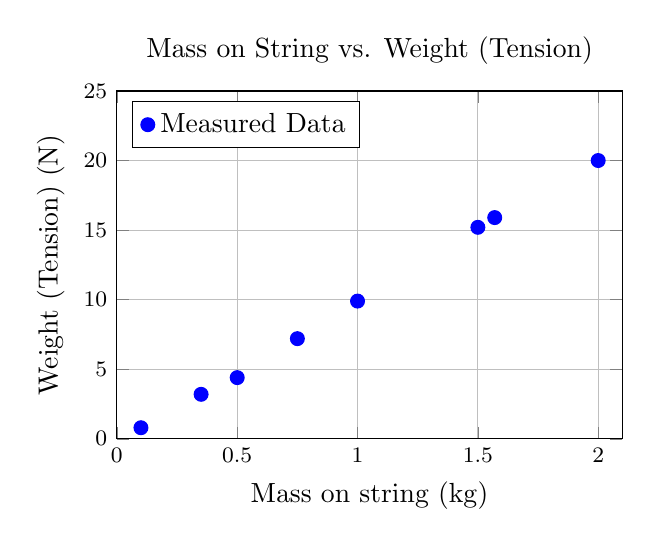
\begin{tikzpicture}
\begin{axis}[
title={Mass on String vs. Weight (Tension)},
xlabel={Mass on string (\unit{\kilo\gram})},
ylabel={Weight (Tension) (\unit{\newton})},
xmin=0, xmax=2.100, 
ymin=0, ymax=25,
xtick={0,0.500,1.000,1.500,2.000},
ytick={0,5,10,15,20,25},
grid=both,
legend pos=north west,
every axis label/.style={font=\normalsize},
every tick label/.style={font=\footnotesize},
width=8cm,
height=6cm,
]
\addplot[only marks, mark=*, mark options={scale=1.25}, color=blue] coordinates {
(0.100, 0.8)
(0.350, 3.2)
(0.500, 4.4)
(0.750, 7.2)
(1.000, 9.9)
(1.500, 15.2)
(1.570, 15.9)
(2.000, 20.0)
};
\addlegendentry{Measured Data}
\end{axis}
\end{tikzpicture}
\end{center}
\caption{\label{fig:mass_tension_graph} Graph showing the roughly linear relationship between the mass on the string and the measured weight (tension).}
\end{figure}




        
    
\section{Discussion}

Our results indicate that as the mass on the string increases the measured tension also increases in turn, confirming Newton's first law (\cref{tab:table1}, \cref{fig:mass_tension_graph}). We observed a direct relationship between the mass and tension, as seen in \cref{fig:mass_tension_graph}. As the mass increased from \qtyrange{0.100}{2.000}{\kilo\gram}, the tension rose proportionally from \qtyrange{0.8}{20.0}{\newton}, confirming the predictions based on Newton's first law since the tension increases. The data is closely aligned with theoretical values of the weight force, showing consistent accuracy in the result. Minor deviations observed were due to to friction in the pulley and calibration imperfections in the spring scale, but had minimal impact on the overall trend. Overall, the findings support that, under constant gravitational acceleration, tension increases with mass. 
      
Despite our attempts to simplify conditions, some factors may have affected our results, such as friction between the pulley and string (see \cref{fig:setup}) and slight differences in the expected and actual weights. Misalignment or reading errors with the spring scale may have also introduced inaccuracies. To reduce these issues in future experiments, recalibrating weights and lubricating surfaces would reduce the experimental error.
        
Overall, the results highlight how mass and force relate, showing that as mass increases, acceleration decreases under constant force. Real-world conditions, including reaction forces and limitations, should be considered to ensure accurate results.






    
\section{Acknowledgments}
%We thank several anonymous reviewers for their helpful comments on our manuscript. 
%        We thank Alexander Gut and Andrew Barone for their work in data collection and for ensuring the reliability of the results. We also acknowledge Rishith Kilaru and Shrikar Swami for contributing to the experimental design and setup. Special thanks go to Dr. Evangelista for his unwavering support and enthusiasm throughout this project.        
%        \section{Contributions}
%        \hrulefill

We acknowledge the valuable feedback from our peer reviewers, whose insights helped refine and strengthen our paper. AB led data collection and experimental trials; AG assisted with the data collection, trials, and experiment design; RK worked on setup, report formatting, and figures; and SS helped with the experiment design and setup. 
    
%\section*{References}
%\begin{enumerate}
%\item P. A. Tipler and G. Mosca, \textit{Physics for Scientists and Engineers}, 5th ed. (W H Freeman and Company, New York, 2004).
%\item Pelcovits, Robert A., and Joshua Farkas. \textit{AP Physics C Premium, Eighth Edition: 4 Practice Tests + Comprehensive Review + Online Practice (2025).} Kaplan Publishing, 2024. 
%\item Evangelista, Dennis. \textit {Unpublished class notes.}
%\end{enumerate}
\bibliography{lab.bib}
\end{document}